This section is devoted to the investigation of the feedback structure that supports and shapes the system of automobility. \todonote{Perhaps this explanation of \emph{``why cars?''} could be in another chapter: methods? Introduction?}The choice of this particular transport mode is based on two arguments: first, the clear dominance of the automobile as the main mode of transport globally (travel demand) and second, the huge inertia, complexity and stability that the system has historically posed against threats to its dominance, e.g., the 1970s oil crisis, the ``dieselgate'' scandal\footnote{``Dieselgate'' refers to the Volkswagen emissions scandal that started in September 2015, when the U.S. Environmental Protection Agency reported that the German automotive industrial group had been faking emission control tests. This caused the \ce{NO_X} output to be lower in the certification tests than in real-world driving scenarios, thus being able to meet U.S. and European emission standards.} \parencite{guardian2017_Volkswagenrevealsrecord}, or even the 2008 global financial crisis. \fref{f:results:global-passenger-car-production} shows the global production of cars from 1961 to 2015, clearly depicting the effects of the financial crisis, whilst acknowledging that production has kept increasing nevertheless.
%
\begin{figure}[h]
\centering
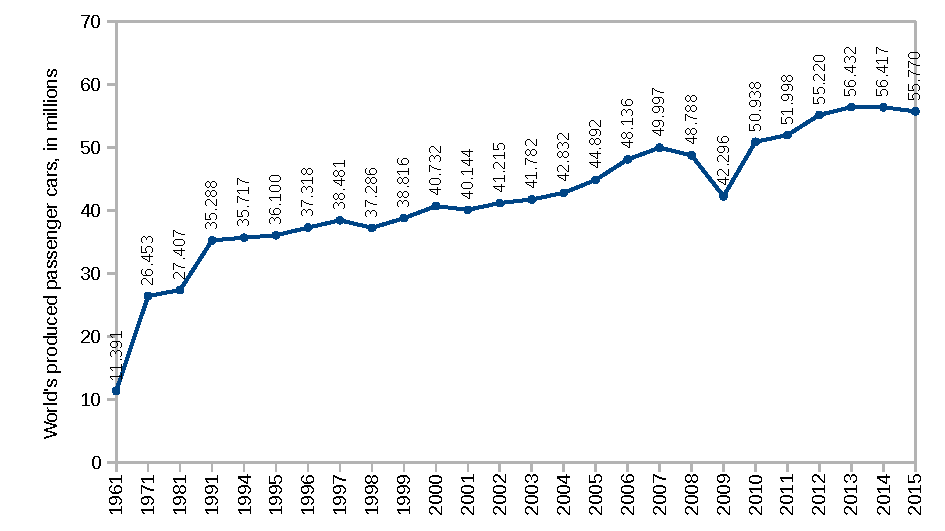
\includegraphics[width=0.8\textwidth]{figures/line_global-car-sales.pdf}
\label{f:results:global-passenger-car-production}
\caption[Global passenger cars production 1961-2015.]{Global passenger car production 1961-2015. Source: own figure; original data from \textcite{bts2017_Table123}.}
\end{figure}

As already mentioned in the \nameref{c:methods} chapter, the study of the feedback structures of the system, detailed in the following subsections, is carried out through a series of Causal Loop Diagrams (CLD). Because of the resilient nature of the automobility regime, the collection of CLDs that form the overview of the system is referred to as the AUTOLOCK model. \ssref{ss:results:cld_urban-planning} discusses the stability mechanisms of automobility from an urban planning (land use) perspective. The cultural basis and legitimacy apparatus of automobility is described in \ssref{ss:results:cld_cultural-feedbacks}. \ssref{ss:results:cld_public-transport-automobility} provides a (partial) explanation of how automobility displaces public transport and vice-versa. Finally, \todonote{Talk about PLPs}

\subsection{Urban planning and automobility}
\label{ss:results:cld_urban-planning}

\begin{figure}[h]
\centering
\fbox{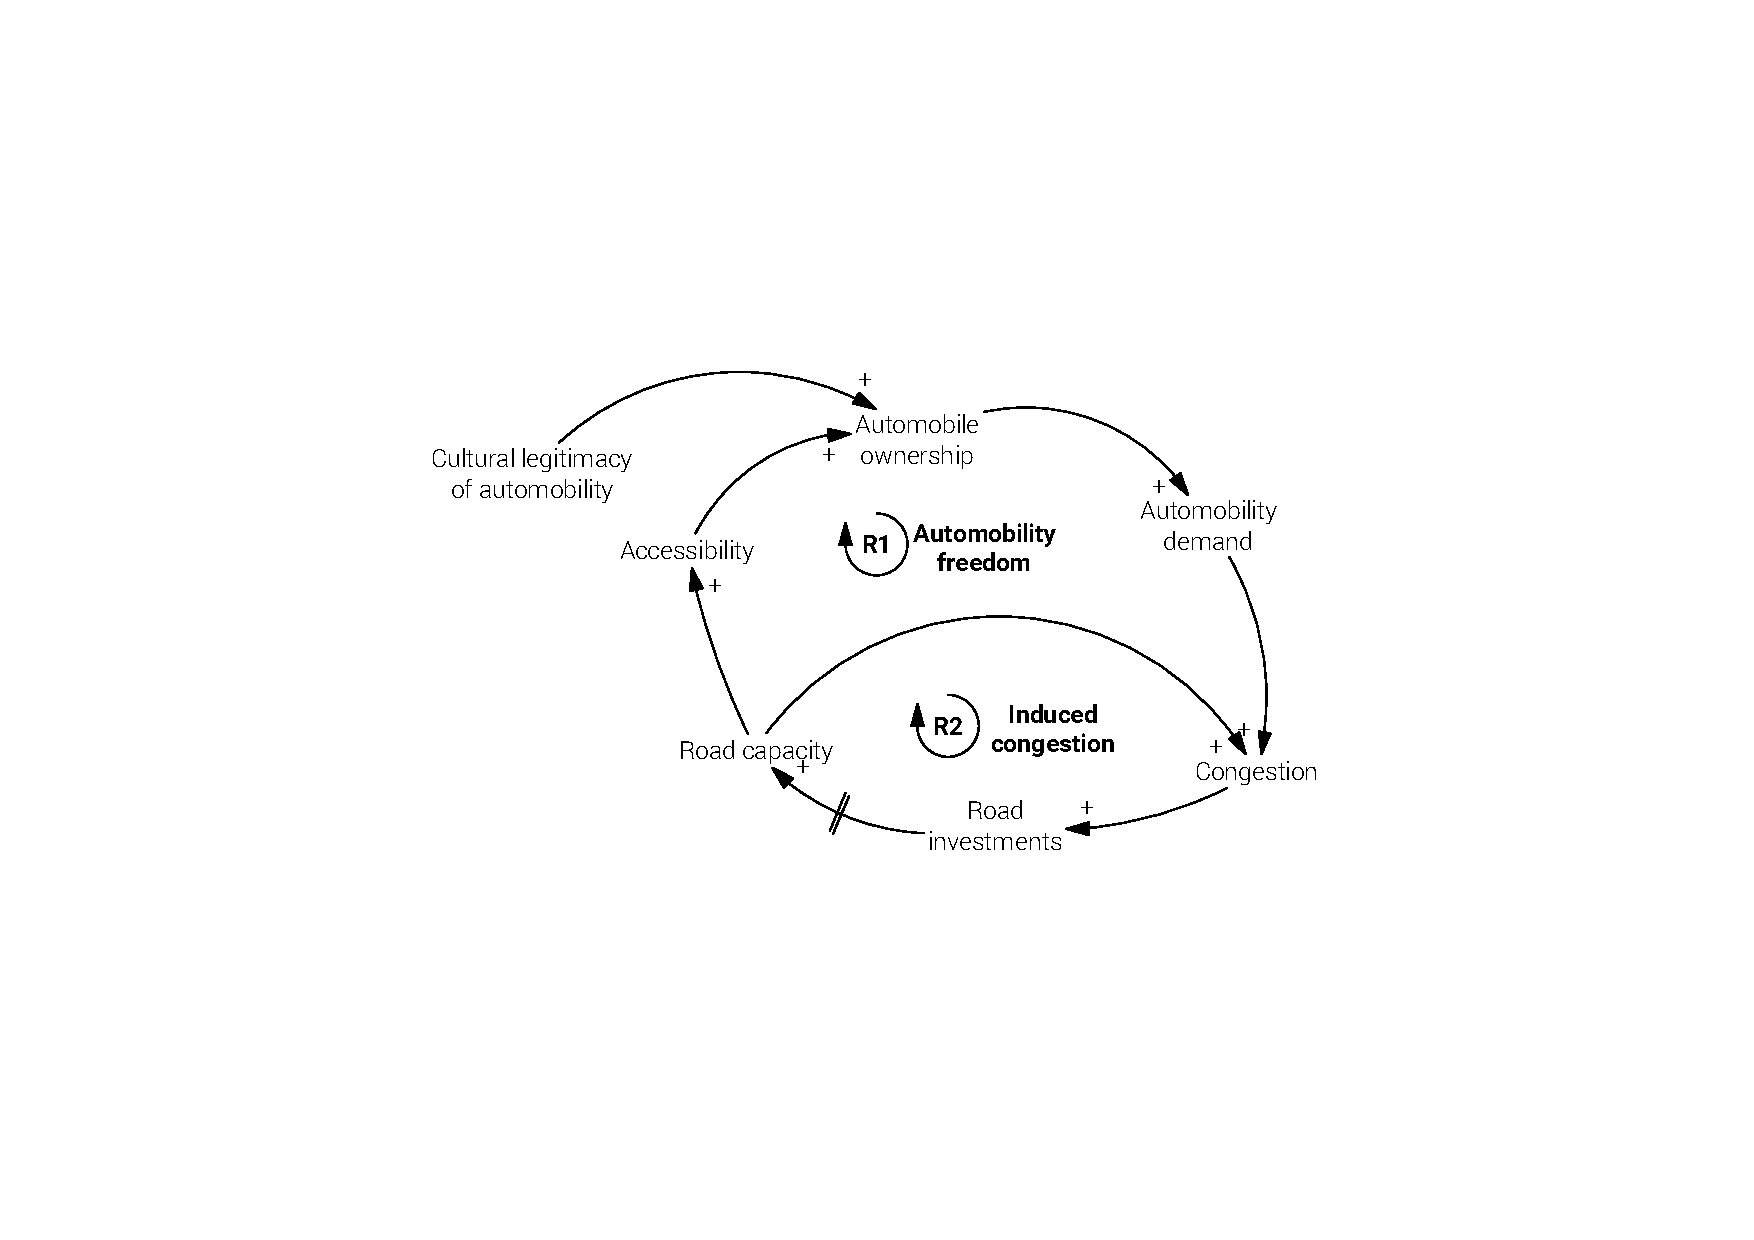
\includegraphics[width=\textwidth]{figures/model/congestion-urban_1_core.pdf}}
\label{f:results:cld_congestion_1}
\caption[]{}
\end{figure}

\begin{figure}[h]
\centering
\fbox{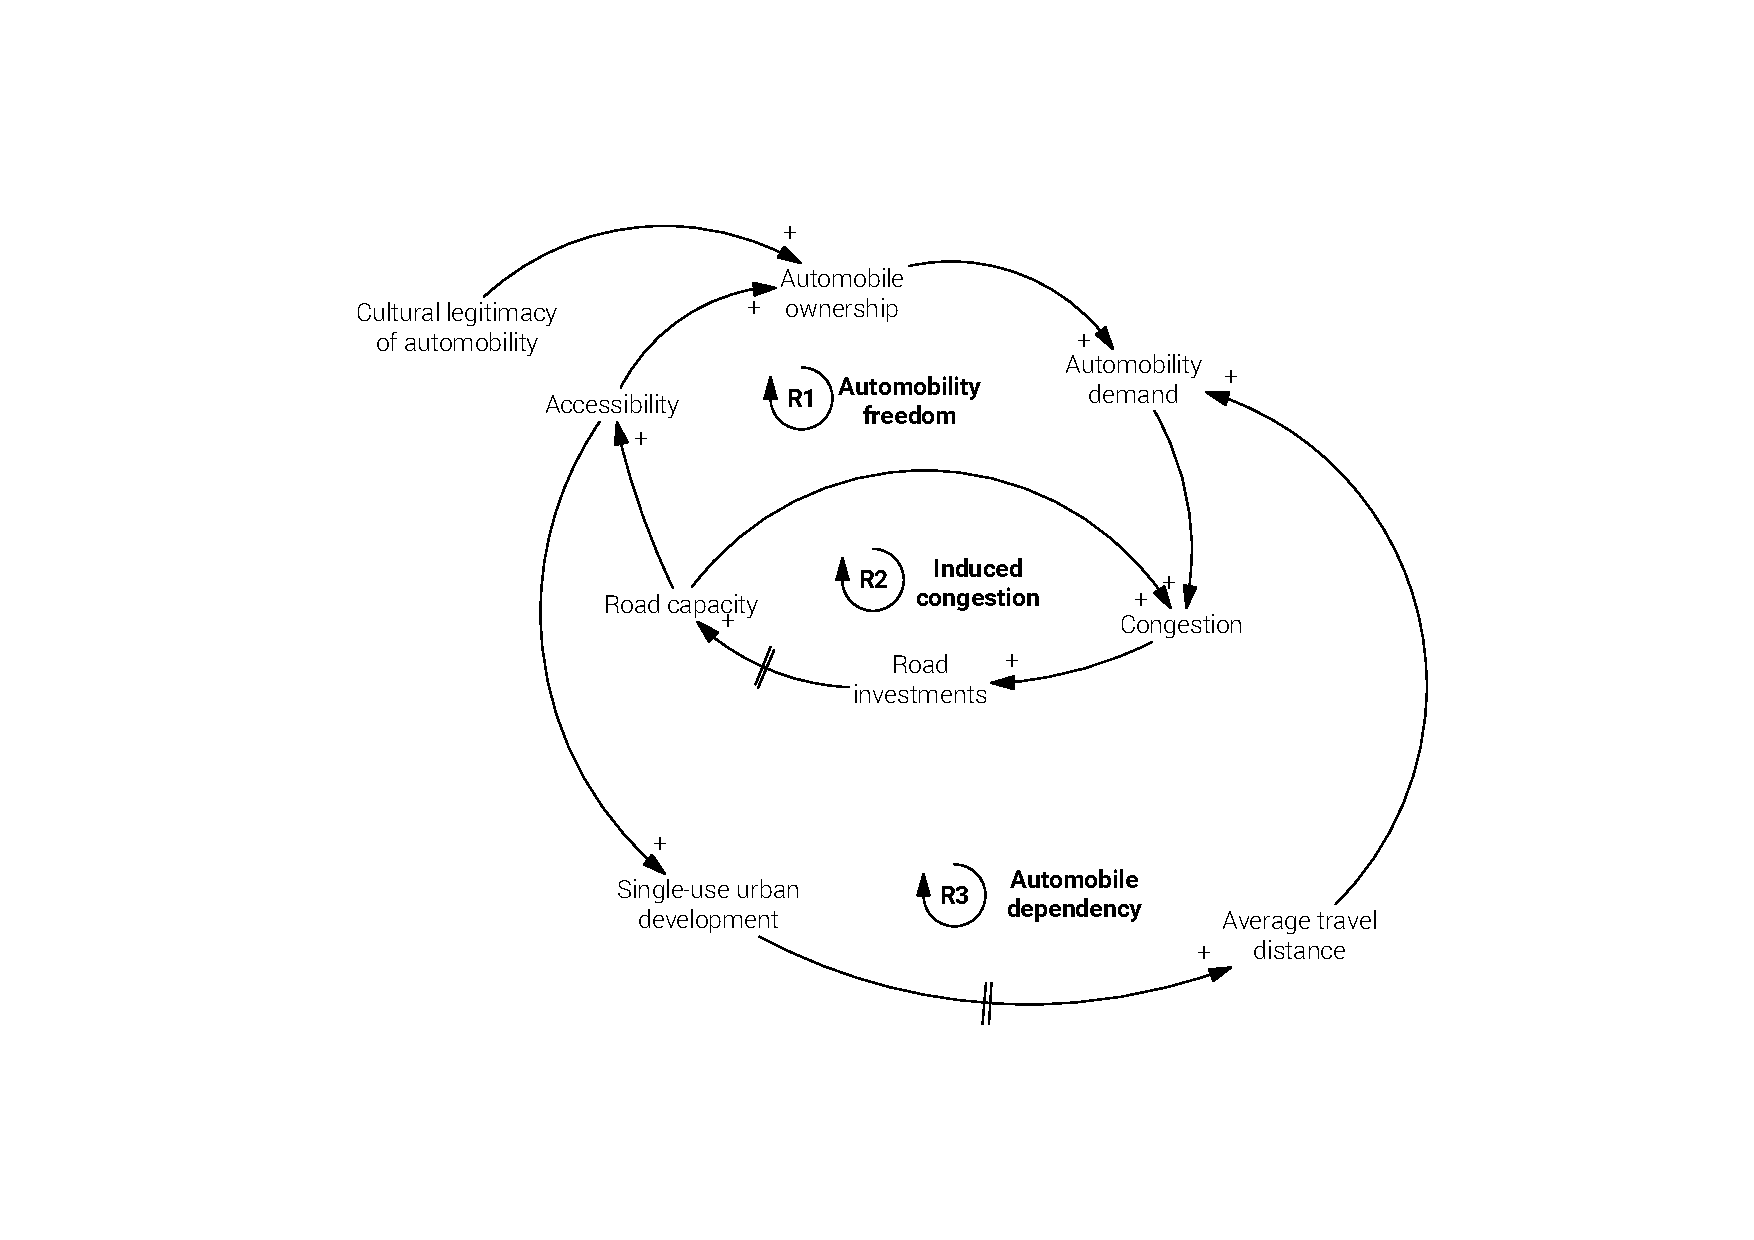
\includegraphics[width=\textwidth]{figures/model/congestion-urban_2_dependency.pdf}}
\label{f:results:cld_congestion_2}
\caption[]{}
\end{figure}

\begin{landscape}
\begin{figure}
\centering
\fbox{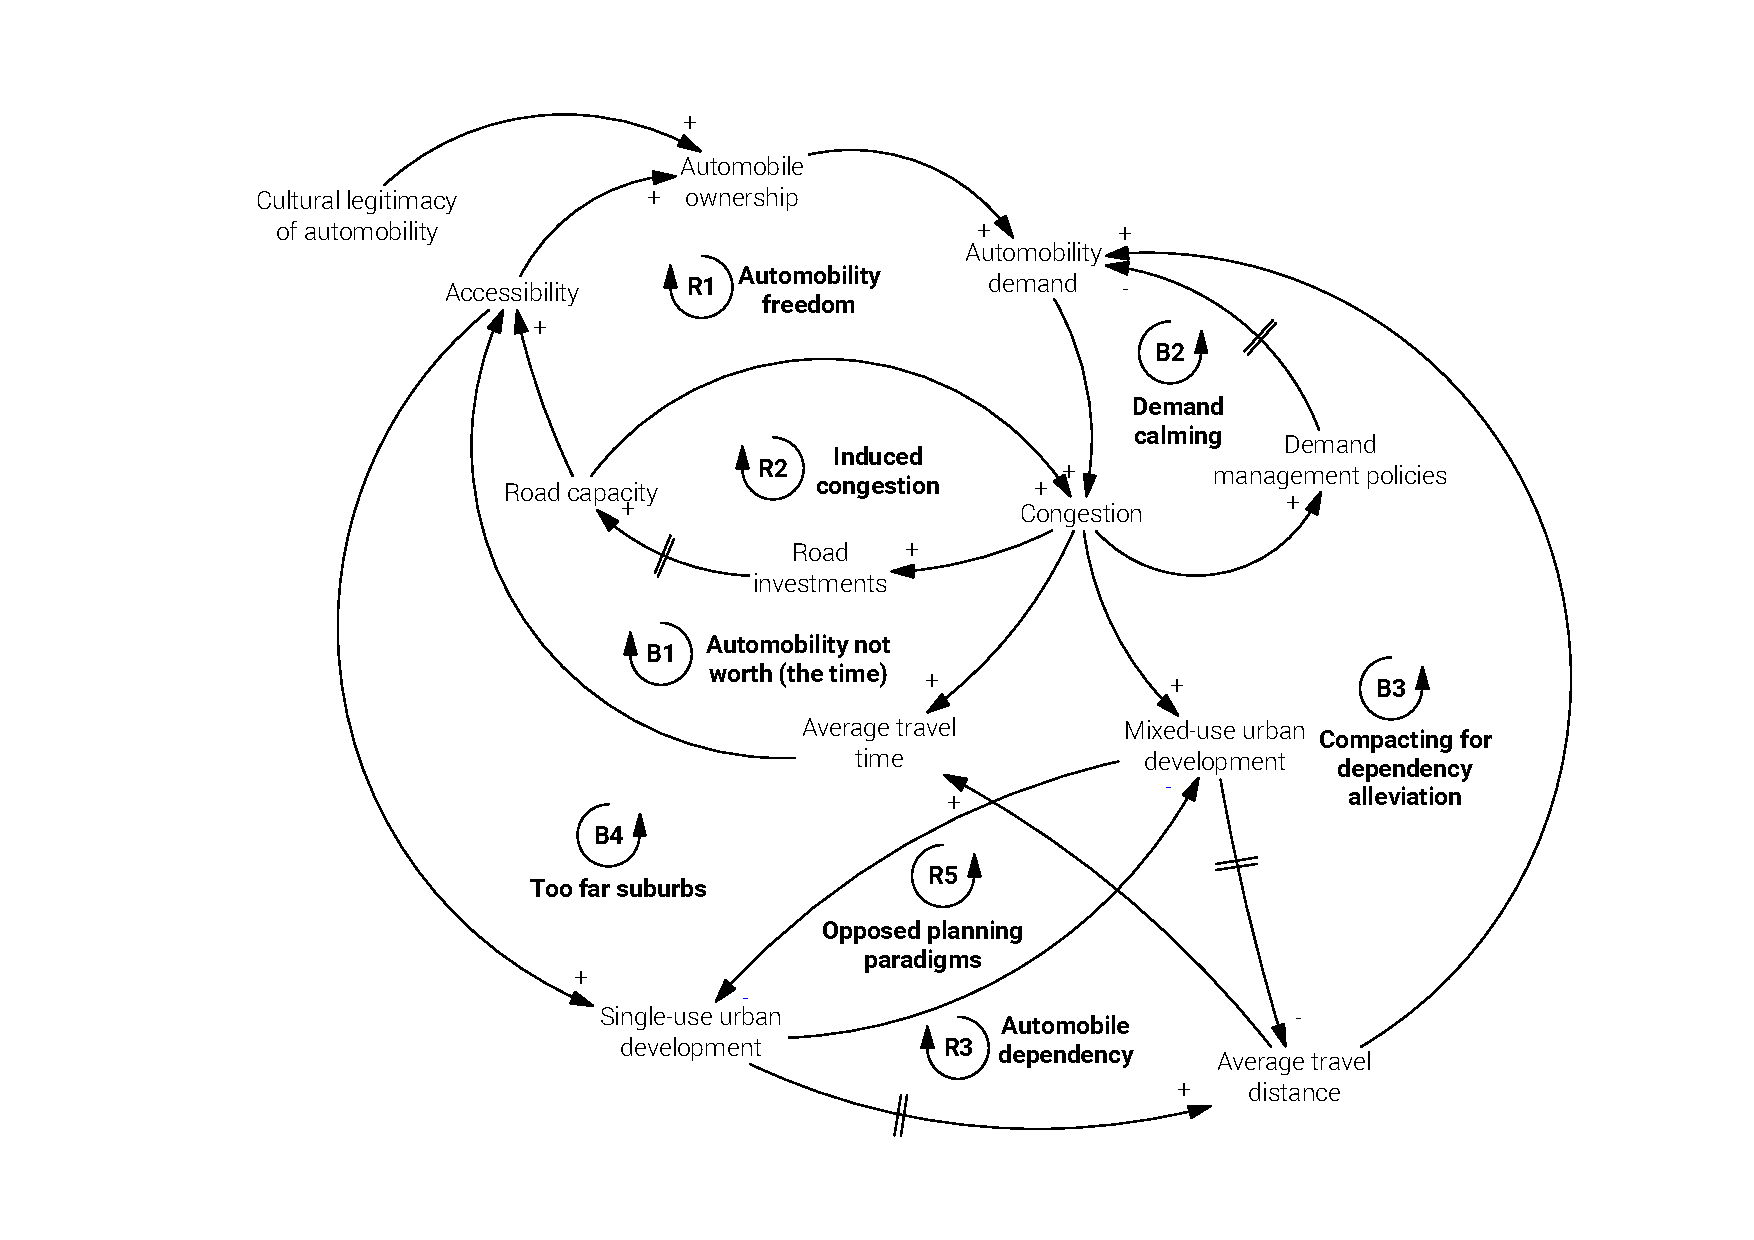
\includegraphics[width=\textwidth]{figures/model/congestion-urban_3_final.pdf}}
\label{f:results:cld_congestion_3}
\caption[]{}
\end{figure}
\end{landscape}

\subsection{Cultural feedbacks}
\label{ss:results:cld_cultural-feedbacks}

\begin{figure}[h]
\centering
\fbox{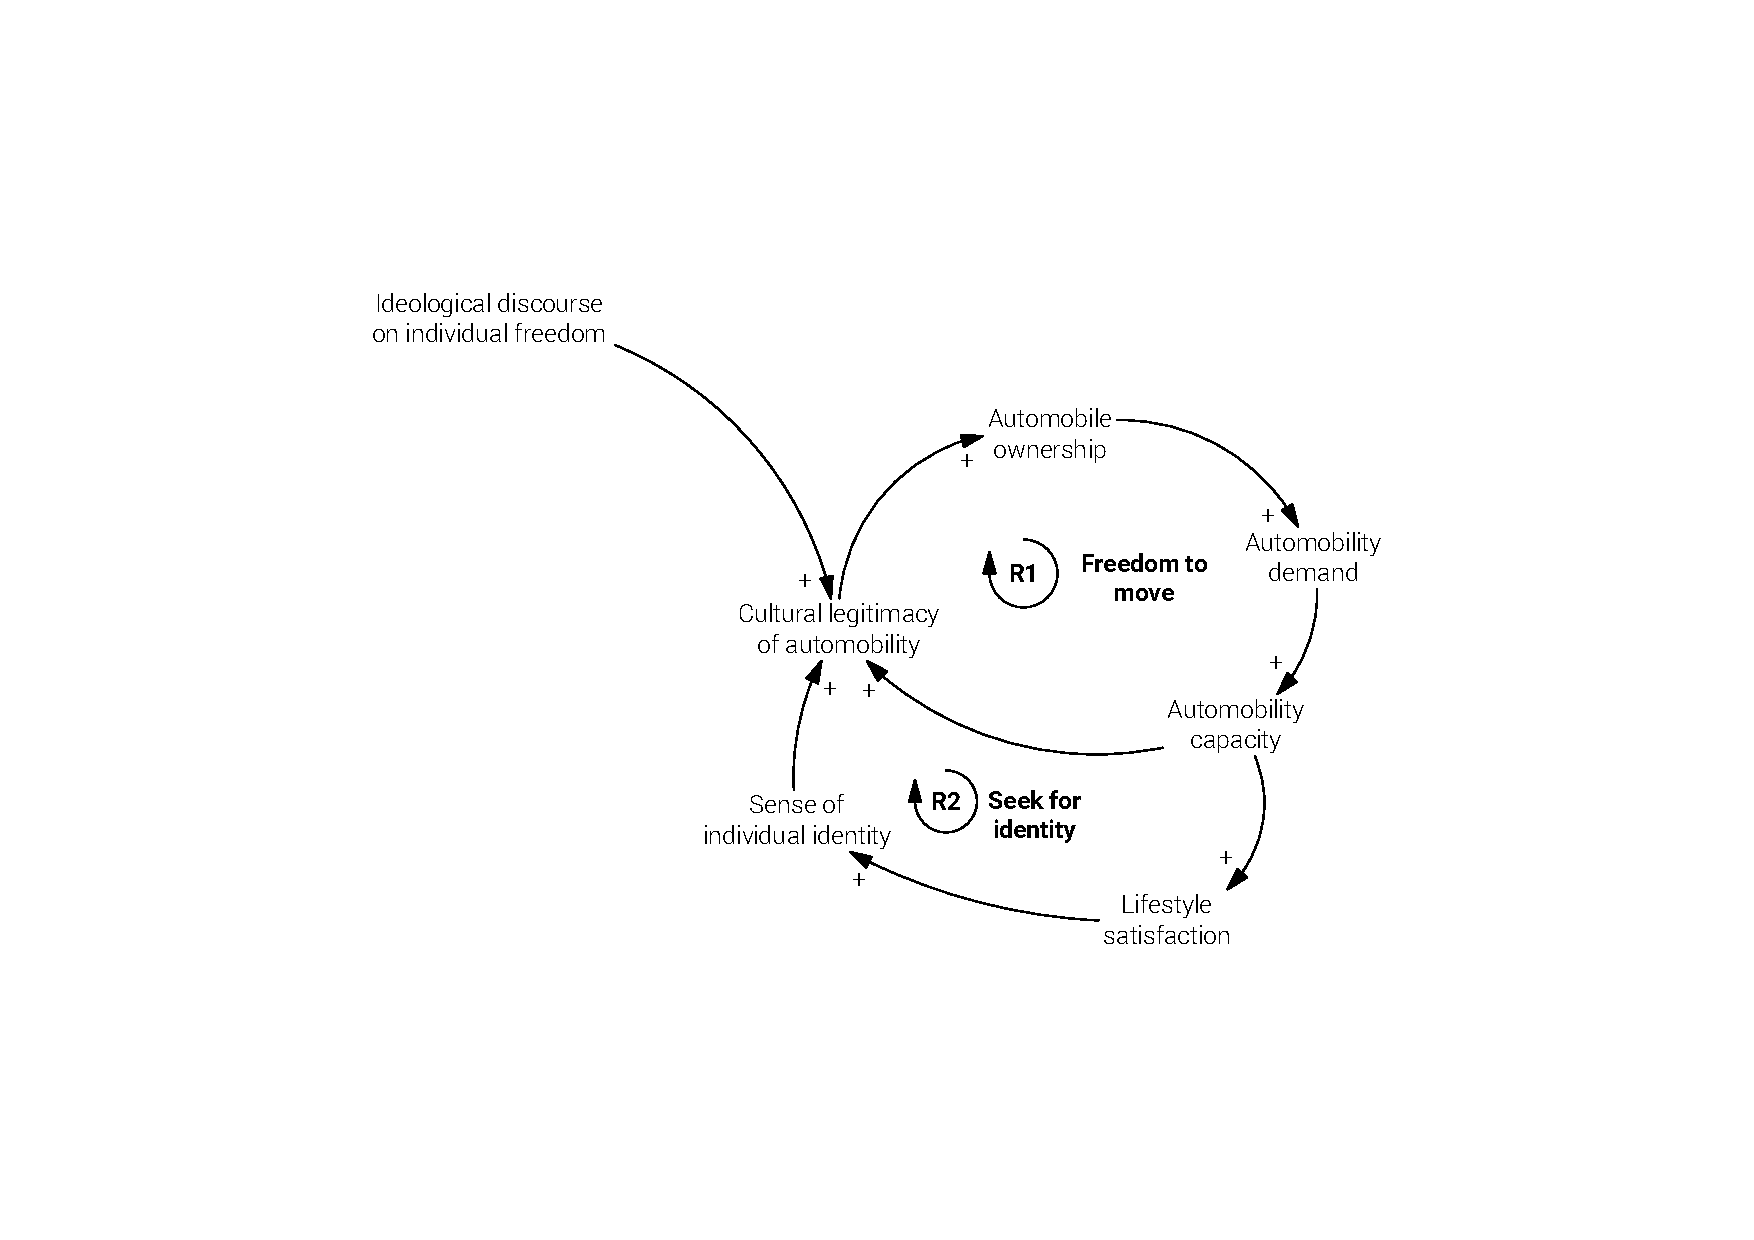
\includegraphics[width=\textwidth]{figures/model/cultural_1_core.pdf}}
\label{f:results:cld_culture_1}
\caption[]{}
\end{figure}

\begin{figure}[h]
\centering
\fbox{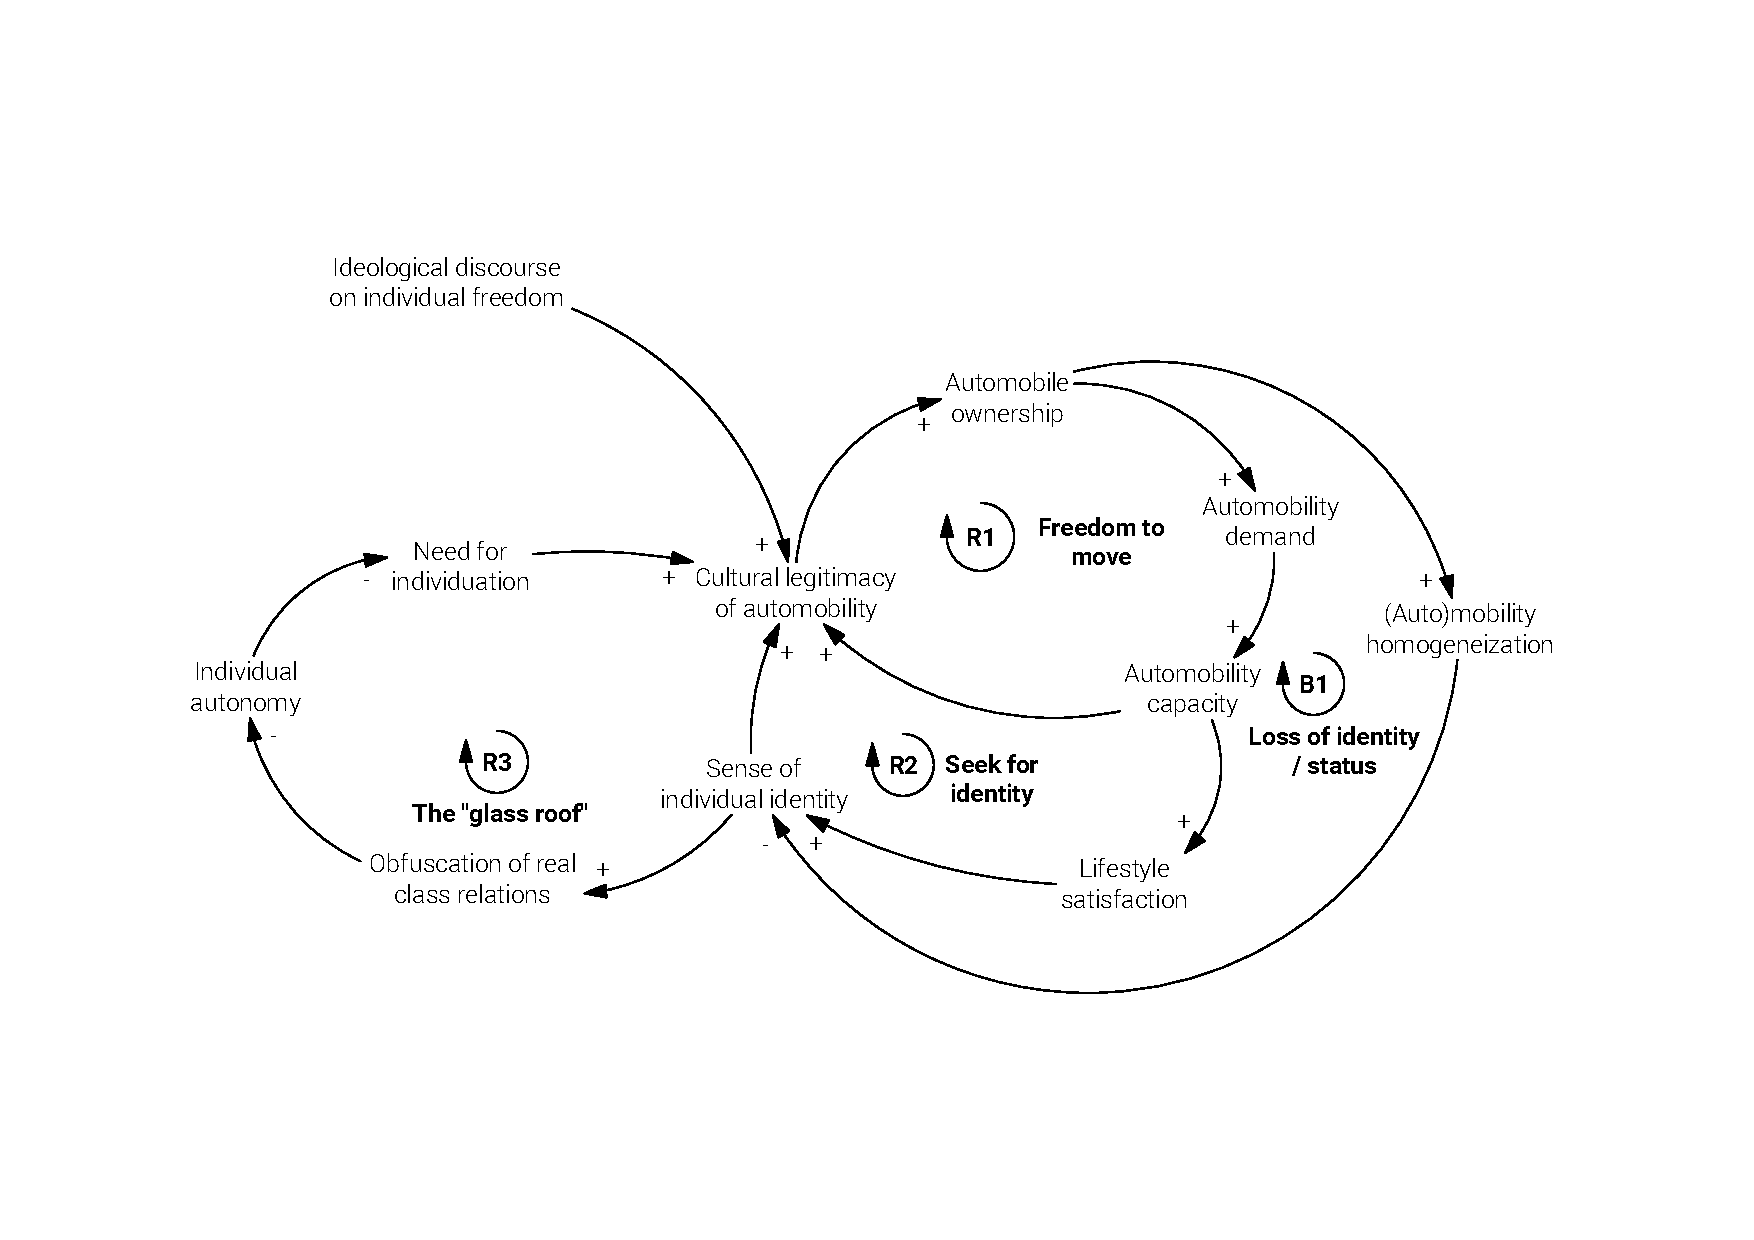
\includegraphics[width=\textwidth]{figures/model/cultural_2_class-relations.pdf}}
\label{f:results:cld_culture_2}
\caption[]{}
\end{figure}

\begin{landscape}
\begin{figure}
\centering
\fbox{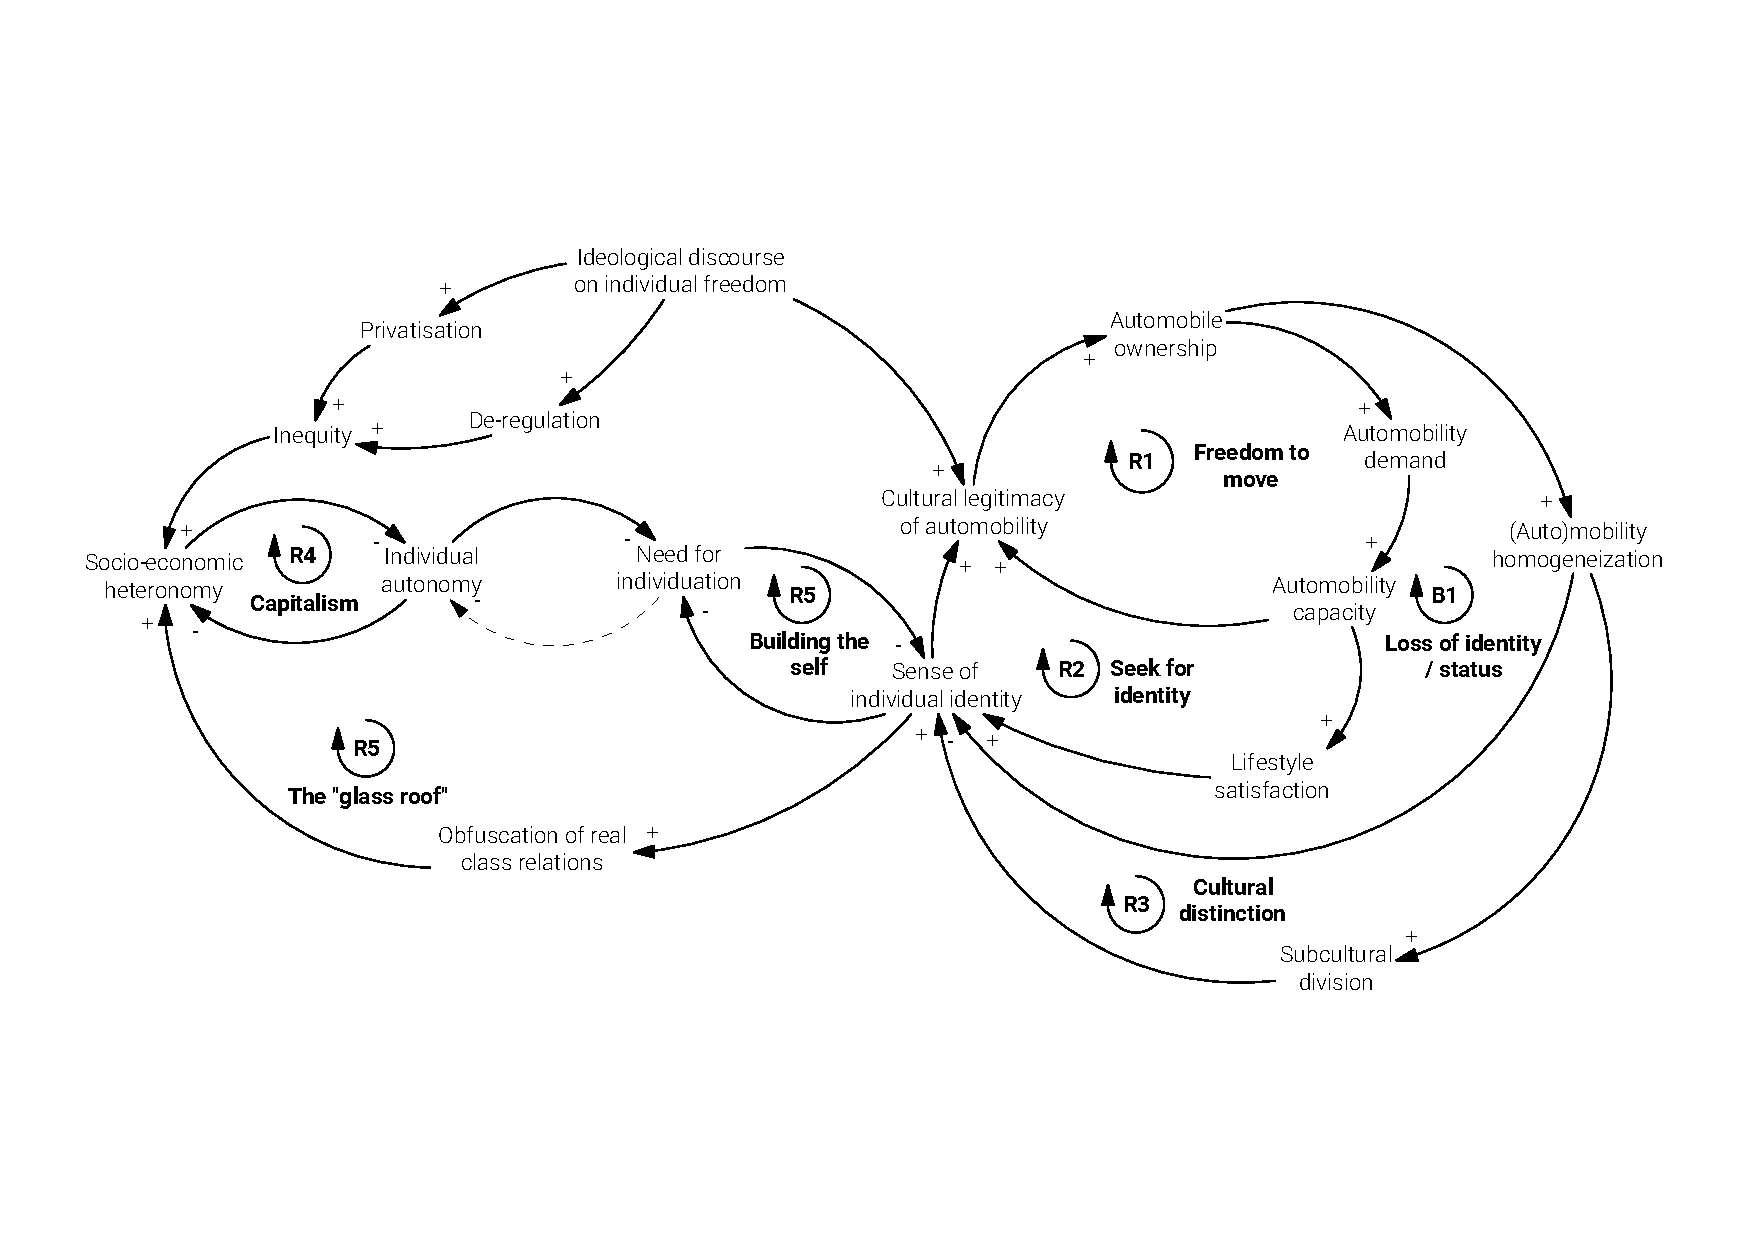
\includegraphics[width=\textwidth]{figures/model/cultural_3_final.pdf}}
\label{f:results:cld_culture_3}
\caption[]{}
\end{figure}
\end{landscape}

\subsection{Public transport vs. Automobility}
\label{ss:results:cld_public-transport-automobility}

\begin{figure}[h]
\centering
\fbox{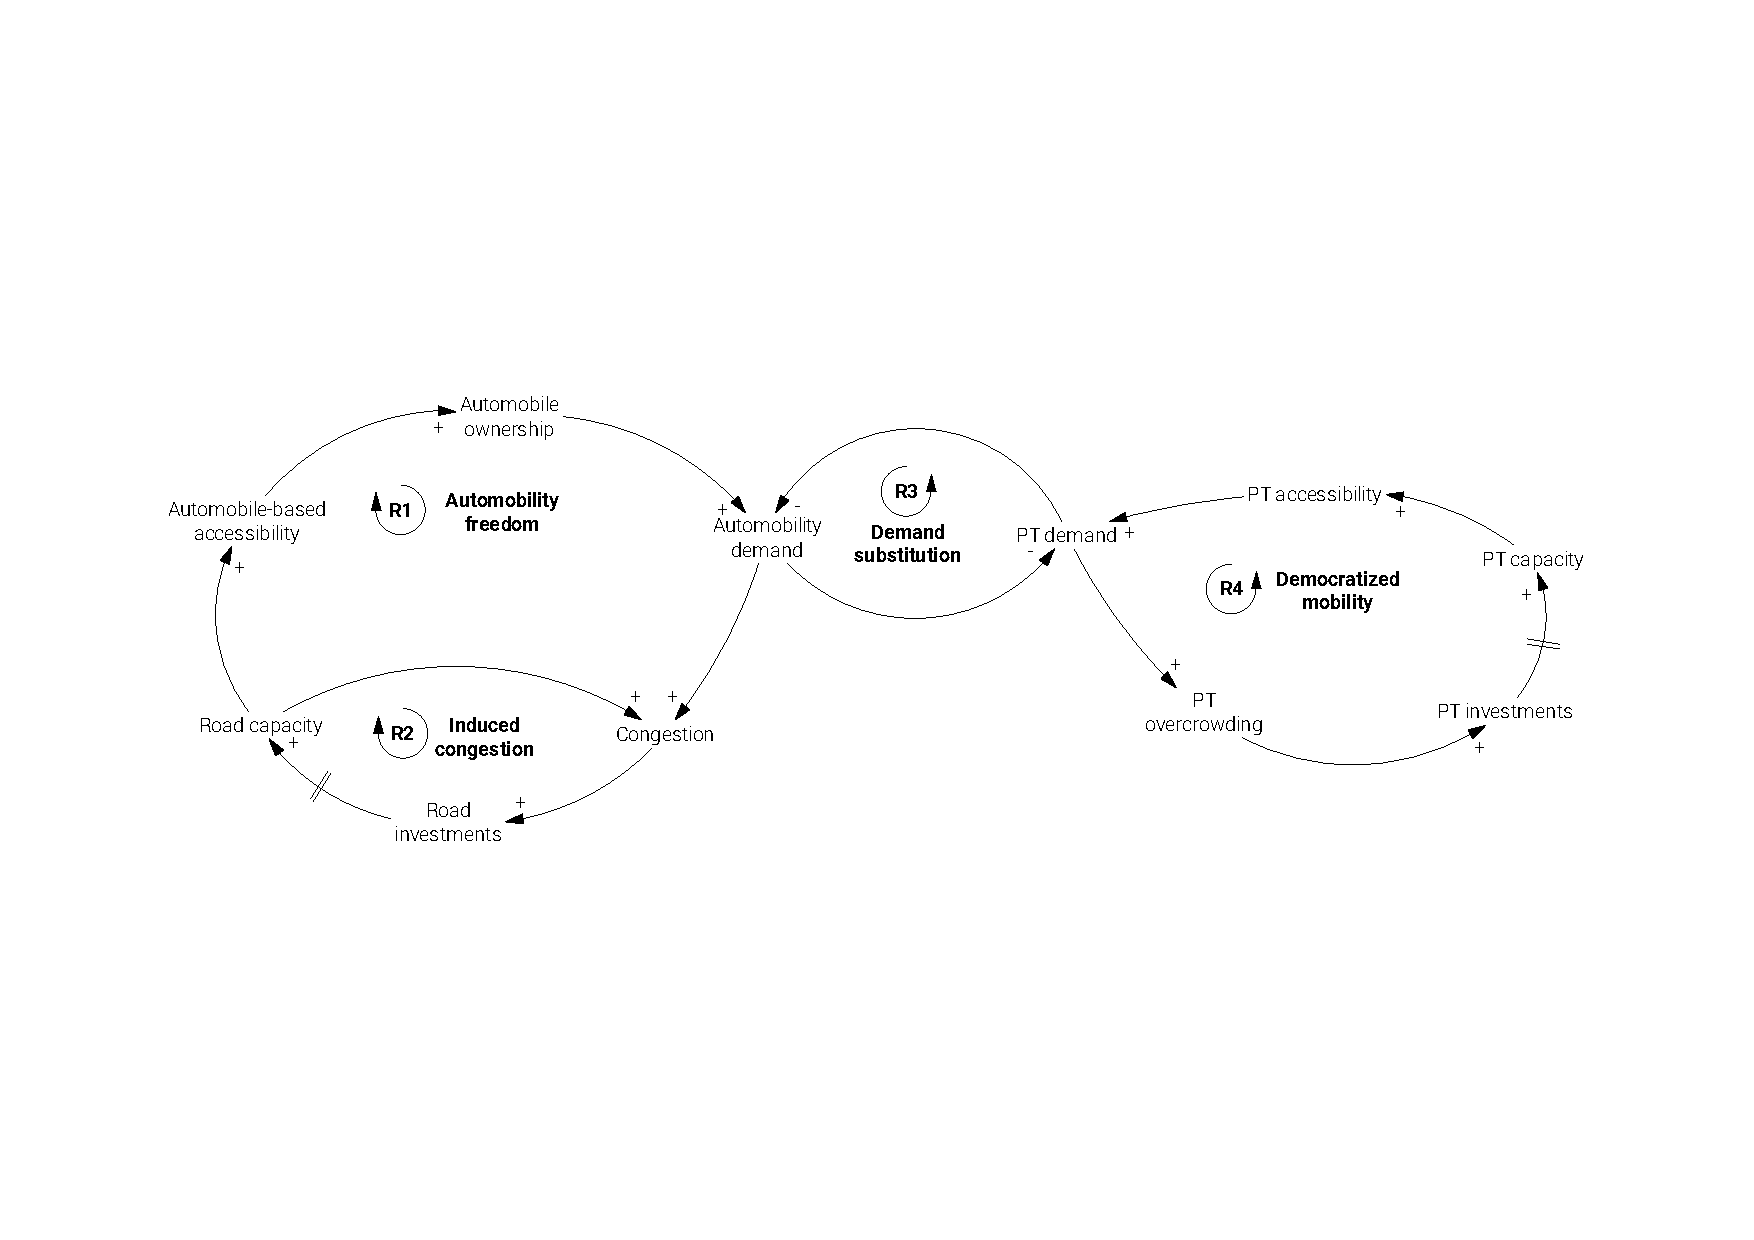
\includegraphics[width=\textwidth]{figures/model/public-transport_1_core.pdf}}
\label{f:results:cld_pt_1}
\caption[]{}
\end{figure}

\begin{figure}[h]
\centering
\fbox{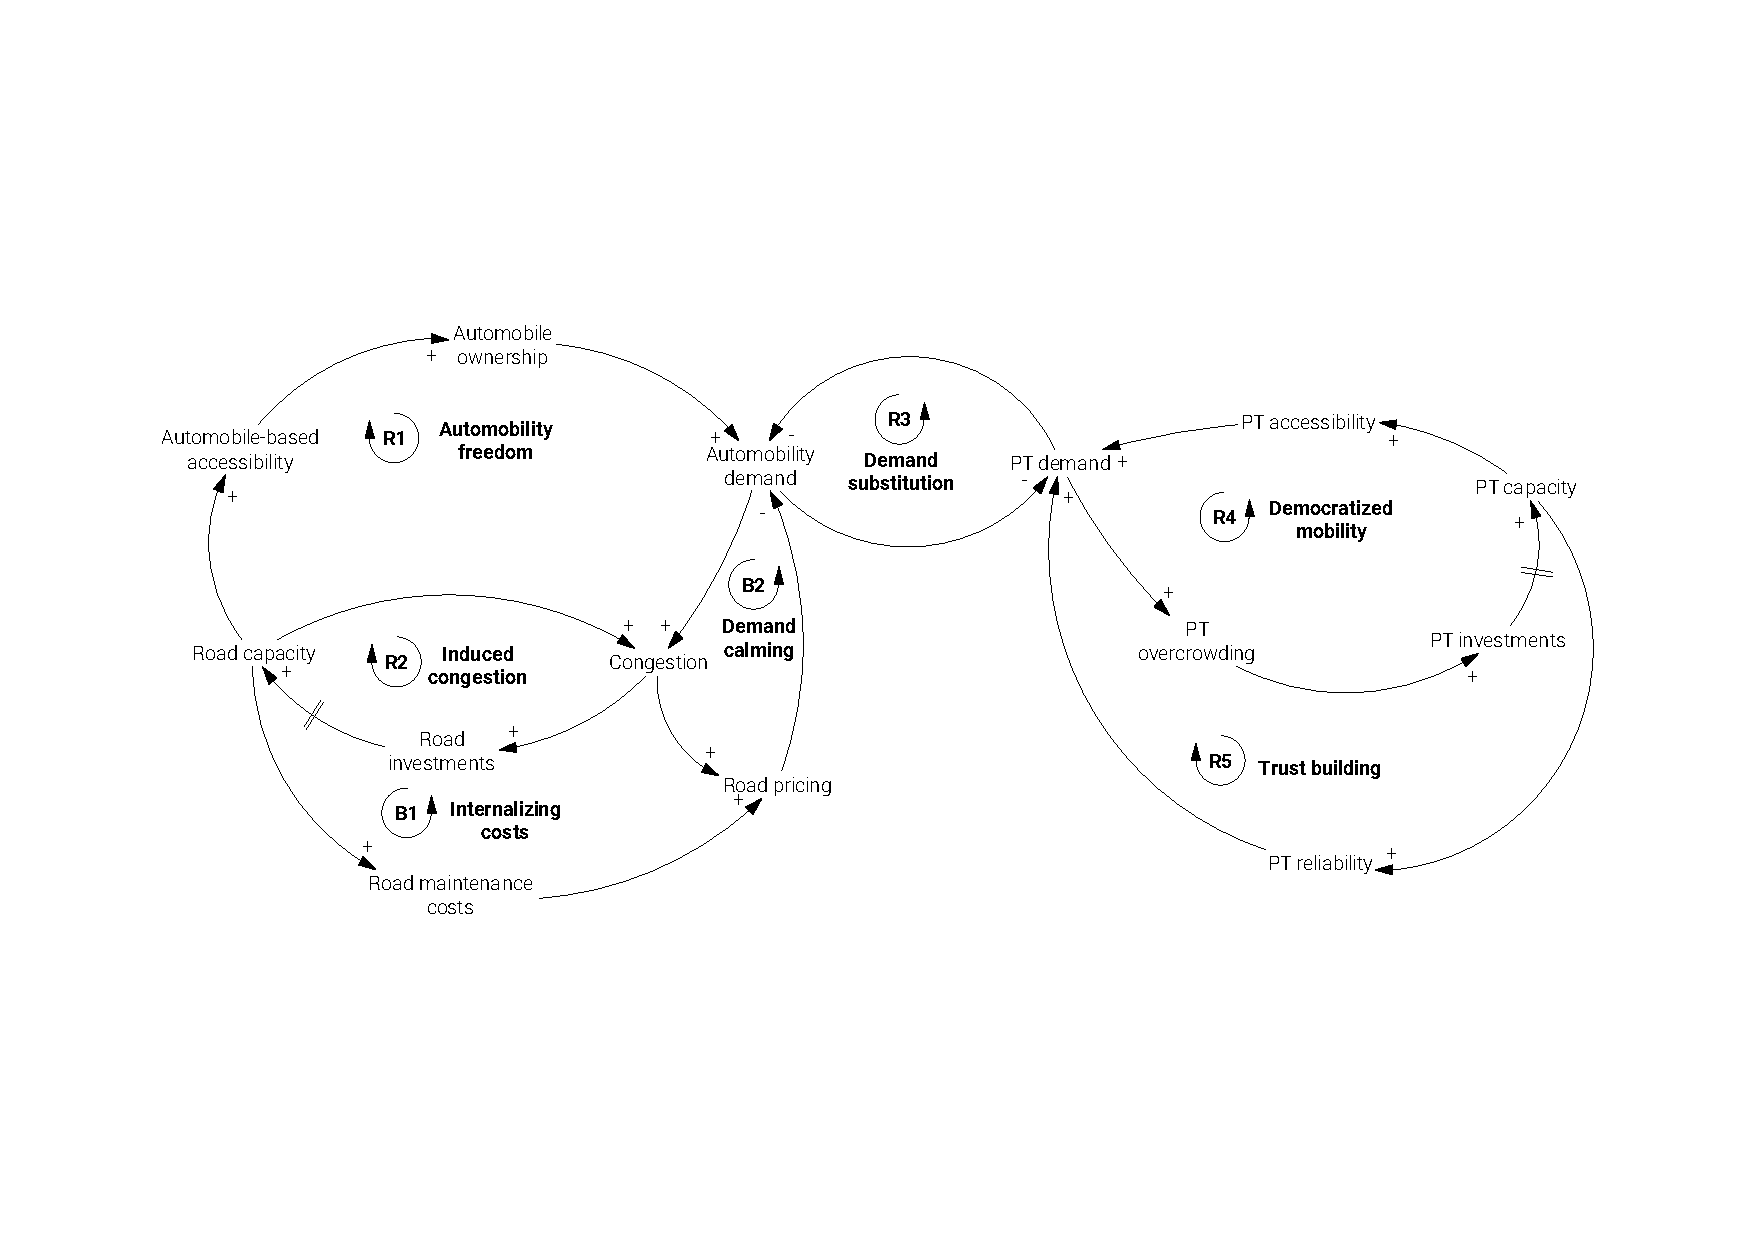
\includegraphics[width=\textwidth]{figures/model/public-transport_2_trust.pdf}}
\label{f:results:cld_pt_2}
\caption[]{}
\end{figure}

\begin{landscape}
\begin{figure}
\centering
\fbox{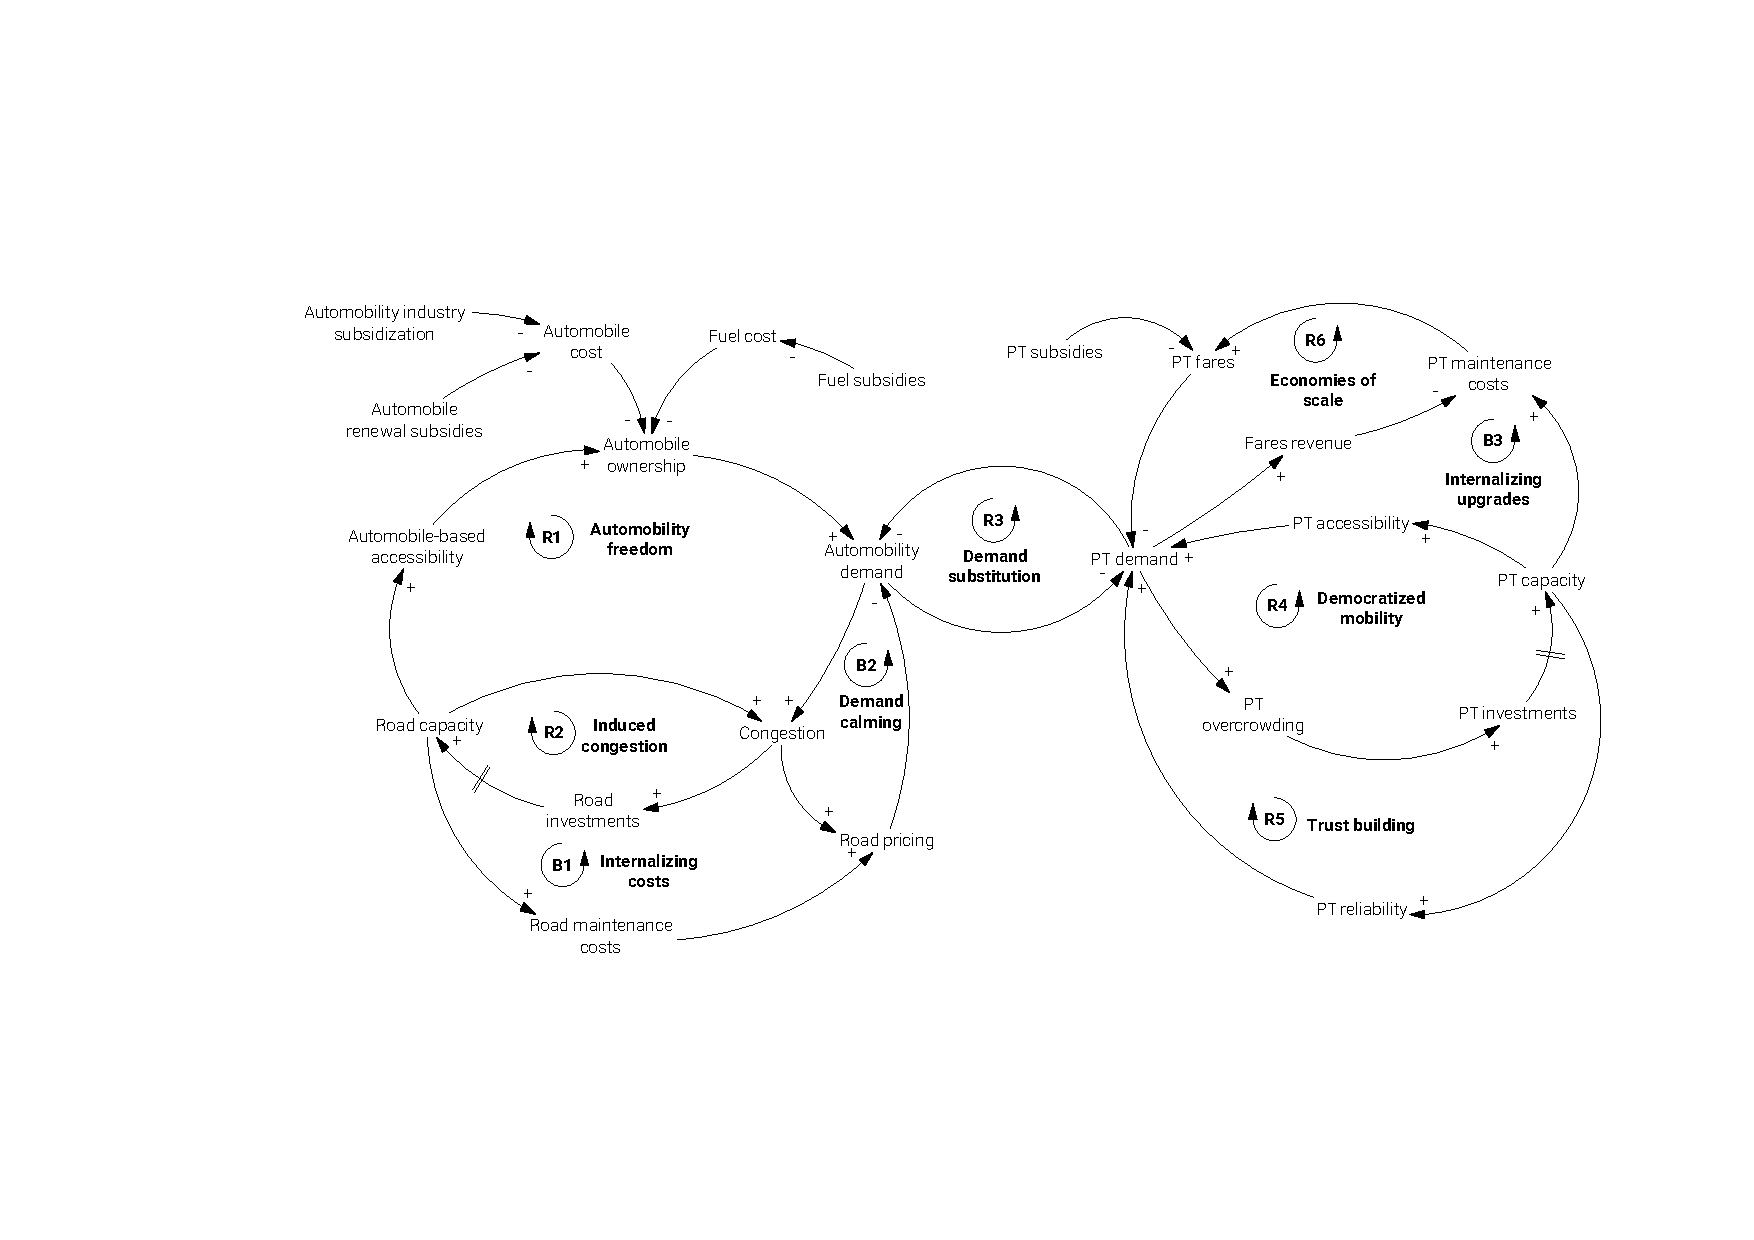
\includegraphics[width=\textwidth]{figures/model/public-transport_3_final.pdf}}
\label{f:results:cld_pt_3}
\caption[]{}
\end{figure}
\end{landscape}

\subsection{Identification of Policy Leverage Points}
\label{ss:results:cld_policy-leverage-points}